\documentclass[11pt, a4paper]{report}
\usepackage{graphicx}
\usepackage{mathptmx}
\usepackage{mathtools}
\usepackage{amsfonts}
\usepackage{setspace}
\usepackage{titlesec}
\usepackage{float}
\usepackage{listings}
\usepackage{color}
\usepackage{caption}
\usepackage{textcomp}

\DeclareCaptionFont{white}{ \color{white} }
\DeclareCaptionFormat{listing}{
  \colorbox[cmyk]{0.43, 0.35, 0.35,0.01 }{
    \parbox{\textwidth}{\hspace{15pt}#1#2#3}
  }
}
\captionsetup[lstlisting]{ format=listing, labelfont=white, textfont=white, singlelinecheck=false, margin=0pt, font={bf,footnotesize} }

\definecolor{lightgray}{rgb}{.9,.9,.9}
\definecolor{darkgray}{rgb}{.4,.4,.4}
\definecolor{purple}{rgb}{0.65, 0.12, 0.82}
\lstdefinelanguage{javascript}{
  keywords={break, case, catch, continue, debugger, default, delete, do, else, false, finally, for, function, if, in, instanceof, new, null, return, switch, this, throw, true, try, typeof, var, void, while, with},
  morecomment=[l]{//},
  morecomment=[s]{/*}{*/},
  morestring=[b]',
  morestring=[b]",
  ndkeywords={class, export, boolean, throw, implements, import, this},
  keywordstyle=\color{blue}\bfseries,
  ndkeywordstyle=\color{darkgray}\bfseries,
  identifierstyle=\color{black},
  commentstyle=\color{purple}\ttfamily,
  stringstyle=\color{red}\ttfamily,
  sensitive=true
}

\lstset{
   language=javascript,
   extendedchars=true,
   basicstyle=\footnotesize\ttfamily,
   showstringspaces=false,
   showspaces=false,
   numbers=left,
   numberstyle=\footnotesize,
   numbersep=9pt,
   tabsize=2,
   breaklines=true,
   showtabs=false,
   captionpos=b,
   upquote=true
}

\definecolor{gray}{rgb}{0.4,0.4,0.4}
\definecolor{darkblue}{rgb}{0.0,0.0,0.6}
\definecolor{cyan}{rgb}{0.0,0.6,0.6}

\lstset{
  basicstyle=\ttfamily,
  columns=fullflexible,
  showstringspaces=false,
  commentstyle=\color{gray}\upshape
}

\lstdefinelanguage{xml}
{
  morestring=[b]",
  morestring=[s]{>}{<},
  morecomment=[s]{<?}{?>},
  stringstyle=\color{black},
  identifierstyle=\color{darkblue},
  keywordstyle=\color{cyan},
  morekeywords={xmlns,version,type}% list your attributes here
}

\titleformat{\chapter}{\huge\bf}{\thechapter}{20pt}{\huge\bf}
\providecommand{\keywords}[1]{\textbf{\textit{Keywords ---}} #1}

\onehalfspacing
\begin{document}
\begin{titlepage}
\centering
{\LARGE UNDERGRADUATE RESEARCH OPPORTUNITY PROGRAM (UROP) PROJECT REPORT\par}
\vspace{2cm}
{\LARGE Reusable Data Visualisation with Structures and Hierarchies\par}
\vspace{2cm}
{\Large AY 2015/16\par}
\vspace{2cm}
{\Large Department of Computer Science, School of Computing\par}
{\Large National University of Singapore\par}
\vspace {5cm}
{\Large\itshape Ding Xiang Fei\par}
\vspace {0.5cm}
{\small supervised by\par}
\vspace {0.5cm}
{\Large Assoc. Prof.~Martin \textsc{Henz}}
\end{titlepage}
\tableofcontents
\begin{abstract}
Recent innovations in visualisation techniques and concepts lead to a greater demand for novel chart types. Research in fields such as social sciences and data sciences produces more data in order to reveal relational and structural data, and visualisation of these data will help social scientists to gain better understanding. Meanwhile, many tools have been developed for visualisation with more flexible data formats or greater variety in types of charts. These includes Microsoft Excel, Chart.js and $\mathbb D^3$. These systems do not yet support modification and authoring of chart types systematically and clear path of data processing which is crucial in processing relational and structural data into actual visualisation. In this work, we will focus on visualisation of relational and structural data and study the capability of relevant tools, including those we have just mentioned. We then explore a better visualisation strategy and methodology that leverage advantages from various tools and produce flexible, responsive and reusable chart designs and visualisation applications.\par
\keywords{visualisation, structural, hierarchy, observation}
\end{abstract}
\chapter{Overview}
\section{Introduction}
Data visualisation has seen wide application in various scientific fields. The recent interest in data mining and deep learning in data science and social science community leads to growing demand for visualisation of relational and structural data. Unlike traditional data with respect to time series and categories, there can be multiple levels of data and rich hierarchies and relations embedded in the dataset.

One example of such dataset is organisation structures of companies or agencies. A typical organisation chart will then display relations between compartments, numbers of occupants of compartments and roles of compartments. In this case, the structure of input data to organisation visualiser will not be linear in structure, but a tree structures with additional data store in each node.
\begin{figure}[H]
\centering
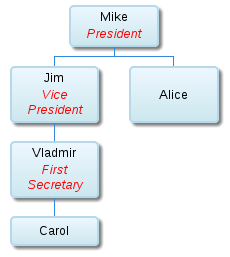
\includegraphics[width=5cm]{fig1_org_chart}
\caption{Organisation chart with Google Chart visualisation}
\label{fig:org_chart}
\end{figure}

\section{Features of Structural Visualisation and Challenges}

We shall now study in details some features of this kind of visualisation. In the context of data science, for example, the input data is usually generated or processed by an external analyser or database. The data in interest ususally falls into at least the following three categories. The first is the data pertaining to single entities which has a list of data attributes, such as volume of trade in a particular year of a certain country. The second is the data pertaining to relations in which two or more entities participate that captures the notion of closeness, difference, change or superiority or suboridination in hierarchy, such as the trade surpluses between any two countries in economic data. The third is the data pertaining to change of values over a time series.

As a case study, we can take one data science research on knowledge landscape of computer graphics as the example. In this research by C., Chen \& R., Paul (2001), the survey of knowledge landscape is done through studying citation and co-citation relationship. After generating necessary information on relations between knowledge concepts, they produce data arranged in a tree structure with each node representing a particular researcher in a field and links representing closeness of specialties between authors. The nodes also contain extra attributes, such as colour to code clusters of authors from the different specialties identified by their algorithms. Traditional cylinder graphs are also placed at each node to represent the number of citations, and they are enabled to vary to show changes over time.\\
\begin{figure}[H]
\centering
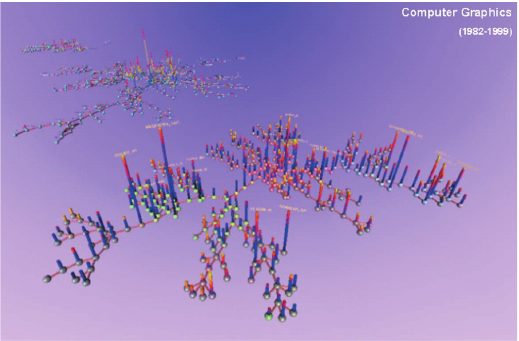
\includegraphics[width=10cm]{fig2_knowledge_landscape}
\caption{Chen, C., \& Paul, R. J. (2001). Knowledge Landscape in computer graphics research}
\end{figure}

The above example captures the three categories of data as mentioned. For single entities, the numbers of citations of each author are encoded by traditional cylinder graphs. However, for data with higher dimensions, they adopt different strategies. In order to encode closeness of specialties between researchers, edges are drawn between nodes and the network graph is further simplified into forests by Pathfinder network scaling algorithm. Colour coding is used to group researchers in similar fields together, which constitutes a relation with many participants. Graphical gadgets such as nodes and vertices are commonly used to display relations as demonstrated by this particular visualisation. Graphical attributes such as colours are used to show relations of even higher dimensions, such as clusters of researchers grouped by their field of specialties.

Here we should be able to identify the challenges of visualisation with structures and hierarchies. Variety of graphical gadgets and attributes like colour codes leads to a greater need for a system to designate graphical attributes correctly and reuse graphical gadgets easily. This need is even applicable to traditional charting as well, as the cylinder charts are repeated on each node in the knowledge landscape visualisation while displaying different values associated with each author. With inputs in this particular research scaling up to large quantity, the process of mapping data to graphical gadgets and graphical attributes must be systematic and reusable in order to create any reproducible visualisation without much human intervention.

A correct visualisation with graphical gadgets also involves a task to correct positioning of the gadgets systematically. In order to display a forest as in the knowledge landscape visualisation, the positions of nodes need to be determined before the positioning information can be sent to their 3D graphics rendering processes. This process will involve invoking other algorithms with input being the structure of the data itself and retrofitting the positions into forms that the other graphics rendering proccess can accept.

Reviewing the features of processes of visualisating data with structures, we should understand that such visualisation application requires a more systematic approach to mapping data into graphical attributes and positioning information before sending to graphics rendering. This part of processing might not be as trivial as that in traditional charts link scattering points and bar charts. In the next section, we will investigate the current commercial and open source tools and explore their ability to meet the requirements of such visualisation.

\section{Current Tools and Techniques}
In this section we will study how currently available tools handle visualisation with structures and hierarchies with special focuses as mentioned in the last section's analysis. Tools in this study includes Microsoft Excel, Chart.js and $\mathbb D^3$.

Starting with Microsoft Excel, which is famous for its widespread adoption and variety of chart types. The standard chart types shipped with Microsoft Excel includes column (bar), line, pie, scatter, area charts and more. These chart types are excellent in displaying chart types that are time-variant or grouped as categories. The data input to these charts are usually severial series of data against one single series of data. The only acceptable formats are cells in spreadsheets, so data has to be arranged in a tabular manner. This mandates end users to extend chart types or create new ones within Microsoft Excel. There are commercial graphing solution working inside Microsoft Excel, such as NodeXL which is capable of drawing complex network graphs, but they must be installed before displaying them. A non-plugin solution to extend existing chart types does not exists as well, as the shipped chart types are fixed. Even though Microsoft Excel is programmable with Visual Basic with Application, no extension API of charting (Application Programmable Interface) is available for end users to modify chart designs and add new graphing gadgets.

Chart.js is a web-based visualisation library that support extension of chart types. It includes chart types from Microsoft Excel. The charts are controlled by their respective classes. Interfaces are provided to end-users to extend the existing chart types to display more visual objects and graphical gadgets used in the original chart classes are also reusable. This makes the creation of new chart types much easier. Those reusable graphical gadgets include the axis creation, scale lines, tool tips, bars and labels, which is used to generate the following weighted bipartite bar chart (Figure ~\ref{fig:ribbon_bar_chartjs}). The definition and application of this chart type will be explained in the later chapters.
\begin{figure}[H]
\centering
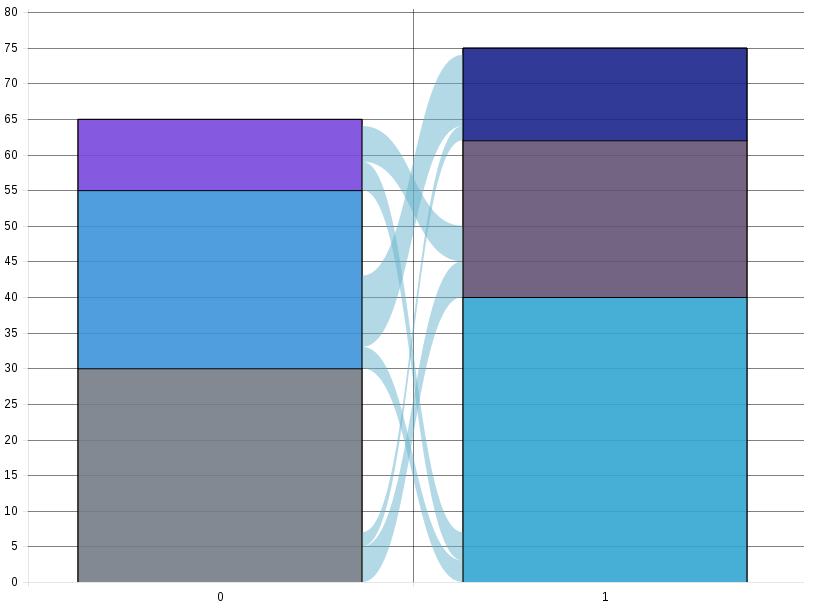
\includegraphics[width=10cm]{fig2_ribbon_bar_chartjs}
\caption{Ribbon bar chart created with Chart.js}
\label{fig:ribbon_bar_chartjs}
\end{figure}
In this figure, a new graphical gadget is introduced to show a relation of flow and it is formed by two Bezier curves on the top and bottom. In order to create this new graphical gadget, the end-user needs to manipulate the underlying native graphics facilities, which is HTML5 Canvas 2D rendering context. This also implies that mapping data (such as the value of a compartment) onto graphical attributes (the y axis in pixels on canvas, with transformation) and calculation of positions (coordinates) has to be done manually.

$\mathbb D^3$ is also a web-base visualisation library. Unlike Chart.js, $\mathbb D^3$ does not work with standalone chart classes, but places more emphasis on data mapping into graphical attributes and configuration of gadgets. The native graphics technology is Scalable Vector Graphics (SVG). Mapping data onto graphical attributes, which can be attributes of SVG configuration, in $\mathbb D^3$ is done by its `data' directive and this binding is one-time and persistent. The structure of the graph and the actual implementation of charts into SVG directives has to be determined by end-user instead, though manipulation of actual structure of SVG is made easier through its tag selection language.

For charts with structures such as network or graphical gadgets like curves and chords, $\mathbb D^3$ works by applying layouts on input data, where the actual positioning of the gadgets are calculated. Again it is the user's responsibility to map the positioning information onto the attributes of the gadgets. Although $\mathbb D^3$ layouts are reusable, as long as the input data has complying format, the graph design itself is not very reusable as the graph design itself is accomplished by user programming as well. Despite of provision of the `data' operator and layouts, variation of data requires manual update on corresponding graphical attributes and positioning in the user program, meaning that the graph design has to be deeply embedded in a program that also processes input data and positioning. It makes separation of the graph design from the user program a potentially painful process. 

\section{Defficiencies and Problems}
We shall conclude some of the defficiencies and problems that current tools possess. Here we identifies two main problems when various user groups can face. First is the reusability issue. We should notice that in most of the systems mentioned above reusability of components is not satisfactory. When in cases user would like to extend the current graphical gadget to show additional information, the gadget design can be entangled with native graphics imperatives (Canvas or SVG in cases of Chart.js and $\mathbb D^3$). In order to reuse the design, the end user has to inspect the processes of visualising the gadgets and transfer the design into his or her application while ensuring the processes remain sound. Since the graphical gadgets are embedded with native graphics imperatives, abstraction of these gadgets can be a challenge when the specification of graphics front-end may not be the same, such as additional transformations needed.

Second is absence of a mechanism to easily map data onto graphical attributes. The need of extra pre-processing of data to extract information, such as positioning done in $\mathbb D^3$ layouts,exacerbates this problem. Data mapping we have encountered so far, even for $\mathbb D^3$ layouts depends on fixed formats and user intervention is needed to transform data into desired formats programmatically. Data mapping onto graphical attributes also have to be done programmatically, which obscures the path of data moving from the original raw data to the actual visualisation output, making visualisation design even harder.

In particular, the second problem leads to another defficiency in aiding end user to design, apply visualisation through interactions. With a fixed chart type and multiple data sets, when end users need to interact and compare different data sets, the visualisation application needs to be manually notified of new data or interactions. Changes to data and therefore changes to graphical attributes are to be also manually notified to the application. It is a common case where end users would like to tweak graphical attributes and configuration for best visualisation effect. The current data binding mechanisms, where data and attributes are bound permanently until further notification, are not responsive enough and, therefore, make the process of design and apply visualisation inefficient.

At the end of this survey on the current visualisation tools, we have identified the two existing problems that make obstacle to visualisation of data with structures. The two problems are reusability of chart components and absence of data mapping and binding mechanism. In the next section, these problems will be solved with new techniques. The solution will focus specifically on the two problems and provide solid foundation for reusable, flexible and responsive visualisations.

\chapter{Solution and Methodology}
\section{Goals}
We will attack the reusability and data mapping issues as the ultimate goal of this report. In this section, we will attempt to examine the visualisation process closer and identify different user groups, in order to make the solution meet their demands as much as possible. Important components need to be separated, so that we can achieve reusability of these components at each stage of visualisation process. Together with data mapping, we will define a protocol for storing data and processes, injection of data and populating changes of data. By properly sectioning the visualisation process and with a systematic approach to data mapping, graph prototyping will be made possible and end users will be able to describe their visualisation explicitly and declaratively, and also be able to reuse graphical gadgets and data digestion processes for their own visualisation applications.
\section[Study of a typical process of visualisation]{Generic Visualisation Process}
Let us review the process of generating visualisation. Figure ~\ref{fig:pipeline} describes this process. A visualisation application has several stages of data processing.
\begin{figure}[H]
\centering
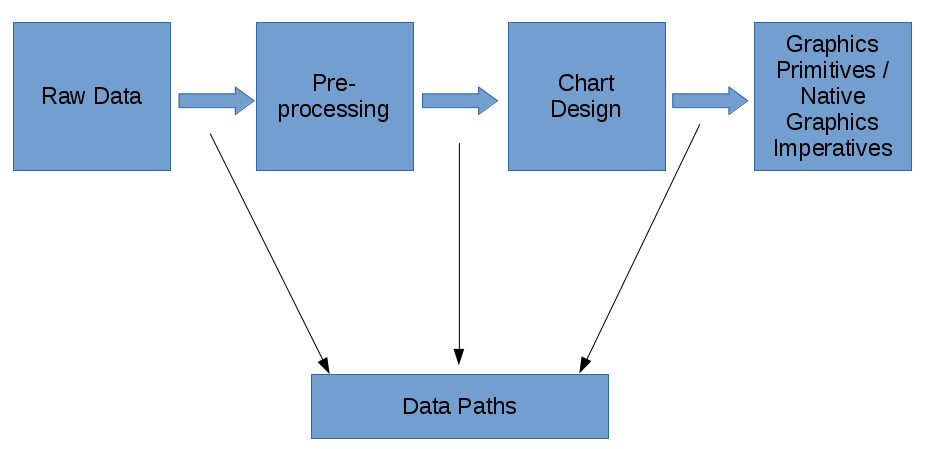
\includegraphics[width=10cm]{fig3_pipeline}
\caption{Visualisation Pipeline}
\label{fig:pipeline}
\end{figure}
A typical visualisation application will have a source of raw data input, and extract data from the structures that visualisation users want to display. The extracted data are then pre-processed and transformed into a format that a chart application can accept. The chart application will then perform further digest on its input, create a collection of gadgets and map the data to their attributes. These gadgets are then transformed into graphical primitives that the graphics front-end is able to display graphics with them. There is a clear data path from the first input to the final graphical output, with user interaction as another input into possibly any of the stages before native graphics stage. 

Each stage is associated with a particular user group with various interests. Figure ~\ref{fig:pipeline_user} explains each of the user groups at each stage. End users with raw data will more concern about how to input their raw data into the visualisation system; visualisation application developer at the second stage will concern about controls on the visualisation system, such as parameters of appereances and interaction, and also about pre-processing the raw data according to end users needs; chart designers will concern about how the input data is further digested into spatial arrangements and configurations of their graphical gadgets; and library writers and maintainers will only concern about providing adequate graphics capabilities and graphical primitives and producing graphics correctly. There is certainly a need for the visualisation solution to separate their demands and address to them respectively.

Putting the tools we discussed in the last section into this context, one can see that Microsoft Excel without plug-ins has fixed pipeline from chart design and graphics primitive; Chart.js does not have data preprocessing stage but an extensible chart design stage; and $\mathbb D^3$ is only working on fixed chart designs, with the given list of layouts, and exposes everything in native graphics imperatives.

The original problem is now reduced to help users focus on each visualisation pipeline stage instead of handling multiples of them at the same time, as well as automate the process of flow of information from one stage to the next.
\begin{figure}[H]
\centering
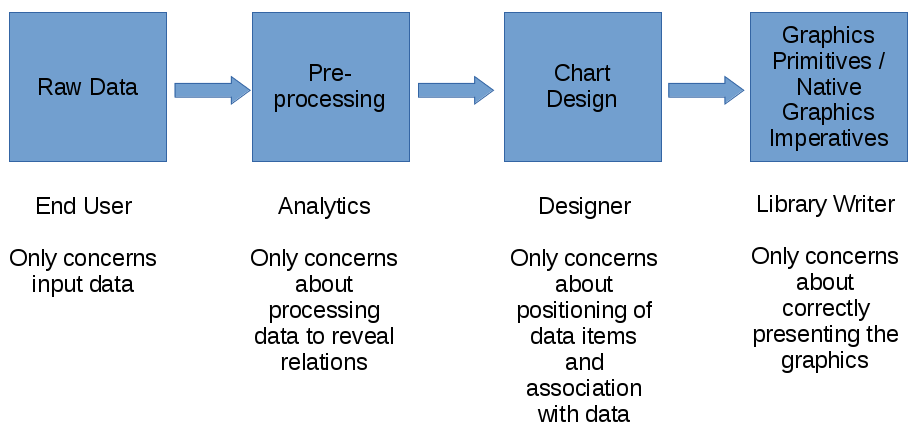
\includegraphics[width=10cm]{fig3_pipeline_user}
\caption{Visualisation Pipeline and User Interests}
\label{fig:pipeline_user}
\end{figure}
\section[Data and process containers]{Organisation and Processing of Data}
In order to facilitate flow of data between the pipeline stages, a protocol is designed as a part of this solution. This protocol defines how data is stored first in some container and populated to other destination. The implementation of the protocol and later the visualisation system is a web-base library written in JavaScript of EcmaScript 2015 standard. Therefore, this protocol is mainly targeted at controlling data flow in JavaScript objects and collections.
\subsection{Shadows}
In this protocol, we define containers of data and processes as models. Models can be either a simple key-value pair storage in form of Javascript `Object' or `Map', or a collection of values of various type in form of Javascript `Array', `Set' or iterable objects. The initial input to the visualisation system and outputs from each pipeline stages can be stored in such models.
\begin{lstlisting}[language=javascript]
var model = {
	series: [1, 2, 3],
	title: 'Sample data model. Values are stored in series.'
};
\end{lstlisting}
In order to make standalone models useful for further processing in other pipeline, model values need to populate through the data path and trigger processing automatically. An operation called shadowing is defined. Shadowing is a process to create another data model capable of observing the target model values for inputs and changes, and triggering data digestion process when inputs and changes are available. The implementation of shadow uses Javascript's Object.observe facility to observe changes to model values.

\subsection{Collections of Values as Shadows}
Collections, such as arrays and any other iterable objects, can also be shadowed. The shadowed collection, just like its key-value pair, is also able to observe key-value pair changes in the target model. In this case, the keys are the indices of the target collection where its values change.

On top of pointwise changes, collections has another type of update operation called splicing. Splicing is an operation to remove elements and insert elements back at a certain position of a collection. One example of splicing on a list of values (`1', `2', `3') is to remove 1 element at the position of value `2' and insert (`4', `5'), and its result is (`1', `4', `5', `3'). A shadow of collection will observe such changes in the target collection, and perform the same operation, except with the processed data values.
\section{Data Binding and Responsiveness}
After defining data storage as models and operations to observe models' values, the protocol defines a simple language to select data from the model. With this language, developers and end users can now select and shadow data model in a declarative way. Developers and end users will focus on data-processing procedure and specification of inputs and outputs of their own components.

\subsection{Data Selection and Computation}
The following listing shows an example to select and shadow a data model of one key-value pair. Suppose that the previous pipeline has one data model `target' as a container for its output of data processing. This stage of pipeline can create a shadow of the input data model, define processes to manipulate the input data and use the shadow as its output data model.
\begin{lstlisting}[language=javascript]
var target = {
	value: 0	// the data value `value', accessible by the expression `value'
};
var context = new el.shadow.ShadowContext;
var shadow = el.shadow.object(
	new Map([
		['shadowed_value',	// store `target's' `value' into `shadow's' `shadowed_value'
		el.shadow.value(context, new el.scope.Scope(target), 'value',
			function (value) {
				console.log('shadow: new value', value);	// demonstrate that shadow observe the change to the data model `target'
				return value;	// return processed value and store into shadow
			})
		]
	]));
// => shadow: new value 0
shadow.shadowed_value;
// => 0
// after some time, target's `value' changed
target.value = 10;
// => shadow: new value 10
shadow.shadowed_value;
// => 10
\end{lstlisting}
When the shadow of `target' is initially created, it immediately takes the latest value of the data model value, which is 0. This value is stored into the shadow immediately. This is also how Chart.js and $\mathbb D^3$'s `data' operator select values from data objects, which is done immediately when data binding is declared. However, this shadow also responds to change in `value' in `target' as well, and then the new value 10 is reported and stored in the `shadow' subsequently.

Simple calculation is possible as well in this data mapping language:
\begin{lstlisting}[language=javascript]
var target = {
	value: 0
};
var context = new el.shadow.ShadowContext;
var shadow = el.shadow.object(
	new Map([
		['shadowed_value',
		el.shadow.value(context, new el.scope.Scope(target), 'value * 10',
			function (value) {
				console.log('shadow: new value', value);
				return value;
			})
		]
	]));
// => shadow: new value 0
shadow.shadowed_value;
// => 0
target.value = 10;
// => shadow: new value 100
shadow.shadowed_value;
// => 100
\end{lstlisting}
Here, the expression `value * 10' means that `value' of target is taken and multiplied by 10 before reported to `shadow' as the new value.
\subsection{Observation}
With this data mapping language, shadows are able to choose portion of data models that will eventually and meaningfully contribute to values that they are observing. For instance, the expression `value * 10' will depend on `value' of the target data model as well as the constant 10. While the expression is evaluated, dependencies of the expression that are variable and traceable are recorded. In this case, `value' is recorded because it is a member of the data model, while the constant 10 will be ignored.

Selective observation allows the visualisation pipelines to respond to only a subset of data changes that the expression is actually dependent at any time. This strategy avoids a full scan of all data models, or also known as `dirty checking', for data changes.
\section{Graph Prototyping}
With shadowing, the configuration of graphical gadgets and computation of graphical attributes can be separated into other processes in the pipeline and their outputs will contain the desired data that is used for arranging and configuring the gadgets. We can leverage this advantage to prototype chart appearance declaratively, so that the structure of the chart is clear and transparent to chart designers.
\subsection{Graph Description Language}
In this visualisation solution, another declarative language is defined for describing chart structures, graphical gadgets and graphical attributes. In the implementation, this language takes the form of XML and JSON as well. The main feature of this language is that it supports data binding from output models or shadows from previous pipeline stages. It provides a subset of graphical primitives for two dimensional canvas that is sufficient to display complex shapes for visualisation with structures.

Here we provide a sample of description of a simple organisational tree diagram in XML flavour, analogous to the one showned in Figure~ \ref{fig:org_chart}. We will show a portion of this chart description where a box with text element representing an department node is defined, and the full version will be included in Appendix ~\ref{sec:appendix:org_box}. This listing shows that there are a rectangle and a text element enclosed by a group element, with transformation applied to the rectangle and the text. These basic primitives form a graphical gadgets which will then be replicated elsewhere.

\begin{lstlisting}[language=xml]
<template data-bind="org_box">
	<relative-layout
		data-bind-x="
			/* enable interpolation animation
			of expression `width / 2 - 25' */

			*.interpolate(${width / 2 - 25})
			.with(*.math.cubic_bezier(.4, 1.4, 0, 1))
			.duration(1500)
			.transition"
			y="0">
		<shape
			type="rect"
			data-bind-style="{
				x: 0,
				y: 0,
				width: 50,
				height: 50,
				fillColor: node.color or 'transparent'
			}"></shape>
		<text
			data-bind-x="-$element.textWidth / 2"
			data-bind-y="$element.textSize">
			{{ node.name }}
		</text>
	</relative-layout>
	...
</template>
\end{lstlisting}

\subsection{Data Binding in Graph Description}
Data binding from the input data model into graphical attributes through the special directive `data-bind-'. It contains the same data binding language used for selecting data items and value computation for shadowing between pipline stages. They are used to create another level of shadow models to store the configuration of the graphical attributes, so that during rendering the values are already available and they are only updated when the dependent target models update themselves. Shadow objects are used to improve graphing performance and avoid unnecessary re-computation.

We will explain the data binding use this example. In the listing, we define a group of graphical primitives containing a rectangular shape and a text element. The group has an offset on x-direction by the amount determined by the expression denoted between line 7 and 10, which specifies the value `width / 2 - 25' to be interpolated and animated for 1.5 seconds with a Bezier curve controlling the animation state. The group has a static y-direction offset of 0. The rectangle will have width of 50 units, height 50 units and the fill color is determined by `node.color', which leads the graphic front-end to look up `color' field of a object which is the `node' field of the shadowed model. This `color' value will be used for colour coding. The text will contain a text from the `name' field of the same `node' object. These values will be filled when the primitives are first configured or the target data model updates.
\subsection{Graph with Recurring Structures and Reusable Components}
In order to visualise structures and hierarchies, the graph description language is able to describe graphics with notion of repeats and recurrence. Given the target data model that is iterable, and a pattern to be repeated, the interpreter of this language is able to iterate through the input model and draw the gadgets with each elements in the data model. Using the same organisation tree diagram, we will explain how the graph description language describes a repeating pattern. The following listing is an excerpt from Appendix ~\ref{sec:appendix:org_box}.
\begin{lstlisting}[language=xml]
<template data-iterate="child, index in children">
	<template data-condition="child">
		<template data-model="{
			child_x: index ? offsets[index-1] : 0,
			child_y: 60
			}">
			<!-- recursive -->
			<relative-layout ...>
				<template
					data-inject="org_box"
					data-argument="child"></template>
			</relative-layout>
			<!-- relation -->
			<shape type="line" ...></shape>
		</template>
	</template>
</template>
\end{lstlisting}
This listing describes a chart that will repeats graphical gadgets described from lines 2 to 16, based on elements in `children' of target model. For each children departments of the organisation, we can draw line from the parent department to it to show it is subordinate (line 14).

In addition to iterating through collections, the language also describes recurrences. Graphical gadgets can inject other gadgets, including itself, with additional data models. For example, on line 9 to 11, each department node will inject another department node, along with information on the child department called `child'.

Such control flows are supported in this language to give more control to generation of graphical gadgets. The directive `data-condition' will only generating the graphics inside the template's children when `child' is defined. Control flows like iteration, injection, modeling and conditional declares when and what graphics to render. The graphics rendering process is now more obvious and comprehensible to end users with the addition of control flows.

The features of this graph description language are its declarative approach to defining the input interface through data models, specifications of graphical attributes to be used by graphing front-end, use of data binding directives to automate propagation of data into native graphics and great reusability of graphical gadgets through support of iteration and recurrence. Since the language is transparent, end users may find it very easy to interpret, modify and extend the capability of existing chart types for more complex structures and hierarchies.

In conclusion, a solution is developed with one language to manage and populate data along a path through the visualisation pipeline with all the process of propagation automated and another language to declaratively define graphical features of a visualisation with focus on structures and hierarchies. This report will move on to explain how the implementation is designed to be more extensible and configurable for various target groups.

\chapter{Design Patterns}
In this section, the design decisions and patterns of the implementation will be explained. From a high level view point, the architecture of the implementation consists of five components: Language Interpretation, Graph Interpretation, Chart Controllers, Observation and Data Patterns.
\section{Design Decisions and Architecture}
There are three tiers of components in the implementation. At the lowest tier lies Language Interpretation, which is the foundation of this visualisation system, which is reponsible for interpreting the data modeling language, computation of expressions and declarations, as well as replay of data dependencies of expressions. This component is also reused internally to describe and execute processes to digest data at intermediate stages.

One level above Language Interpretation is Observation and Data Patterns. Observation is a set utilities to apply observations, create shadows and dispatch change notifications. It is the essential component of the implementation of shadowing. Data Patterns are patterns operating on data models and shadows to perform simle and common operations, such as folding, mapping and counting. There are also patterns used for interpolation between changes of data model values, an important operation to implement any kind of transition animation in visualisation. They provide support for the working of data path protocol and allow reuse of collection operation patterns that many chart applications need.

On The top most level, there are Graph Interpretation and Chart Controllers. Graph Interpretation is a set of utilities to interpret graph descriptions, generate native graphics imperatives and produce the actual graphics output. Chart Controllers represents pipeline stage at chart design, which controls output data models for graphical gadgets. To produce visualisation of choice, end users will just need to choose a Chart Controller, along with its chart description and input data. Little effort is to be done even if the input format does not fit into the Chart Controller's input, as one just need to shadow the original input data object and use the data mapping language to restructure the shadow to retrofit into the desired format.

Following this high level view of architecture, we will next discuss the design patterns used in the actual implementation.
\section{Modules and Functions}
\subsection{Module Factories}
All the mentioned functional components are wrapped into modules with a common facility, so that when connected together in a pipeline fashion, there is a common protocol to retrieve the output data models. This common facility provides additional interfaces to configure gloal or instance settings, instantiate and initialise with proper arguments. For example, after wrapping with this moduluarising utility, all Data Patterns and Chart Controllers expose their interfaces for configurations and a way to retrieve output data models. It is possible then to chain up multiple Data Patterns, or swap out graphics front-end for a different graphics output while keep using the same Chart Controller. This will maximise flexibility and reusibility of the provided tools.
\subsection{Observers}
Shadowing is essentially implementing observation patterns. Shadow controllers evaluate expressions and attach to Observation component according to data dependencies determined by Language Interpretation. In Observation component, change notifications are collected and dispatched to relevant shadowing objects. The observation pattern is used to avoid unnecessary `dirty checking' and it is essential for performance-sensitive components, such as Graph Interpretation.
\subsection{Interpreters}
Interpreter patterns are deployed elaborately in the two language interpreters. A intepreter is a component to walk through inputs and dispatch the data to its relevant sub-intepreter recursively. It is a good pattern to use here as it separates the processes to interpret input data with different semantics and makes the development of interpreter faster and clearer. By using interpreter patterns, future developers can easily extend the languages for more powerful features.

\chapter{Use Cases}
After explaining the methodology, architecture and implementation of the solution, there are two examples with this solution created as a proof of concept. The first one is weighted bipartite bar chart. It is first implemented with Chart.js (Figure.~\ref{fig:ribbon_bar_chartjs}), and is implementated again. The second exmaple is a simple organisation chart, whose chart description has been used to demonstrate the graph description language.
\section{Weighted Bipartite Bar Chart}
In weighted bipartite bar charts (Figure.~\ref{fig:ribbon_bar_chart_vis}), there are iterations of data series to display the volume of compartments. The heights of the individual bars shows these volume data. So far it resembles a stack bar chart design. The additional ribbons connecting a pair of bars across two adjacent iterations visualise the follow of elements or items from on compartment to the other as a change between two iterations. This extra drawing is achieved without any intervention on the native graphics. This is a typical example of display and comparation of data values in a way that reveils relations.
\begin{figure}[f]
\centering
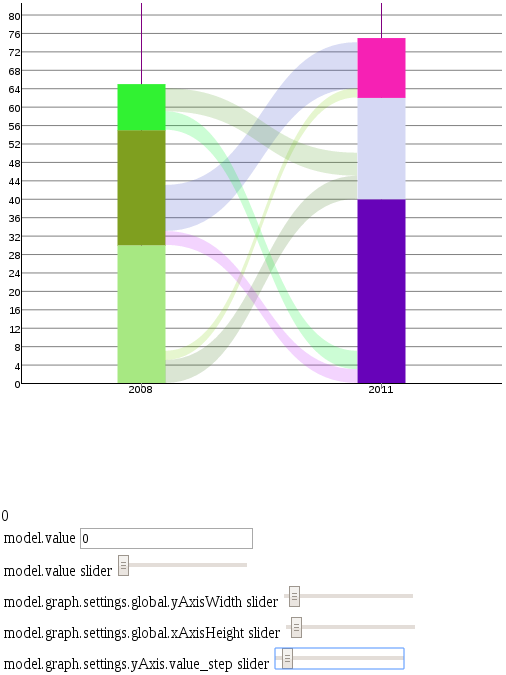
\includegraphics[width=10cm]{fig6_ribbon_bar_vis}
\caption{Ribbon bar chart with our visualisation system}
\label{fig:ribbon_bar_chart_vis}
With shadowing, changes in data and configuration can propagated effortlessly. Below the graphics output region, several control elements exists that are linked to the underlying Chart Controller input data model. Users can scroll and adjust chart parameters and observe effects immediately without programmatical intervention. This can be useful in designing charts as the immediate feedback from graphics output helps users to make design decisions swiftly.
\end{figure}
\section{A Very Simple Organisation Chart}
Organisation chart is another example of visualising structures and hierarchies. In this example, end users input a tree-structured data into this Chart Controller and an animated tree presenting the structure is shown (Figure.~\ref{fig:org_chart_vis}).
\begin{figure}[f]
\centering
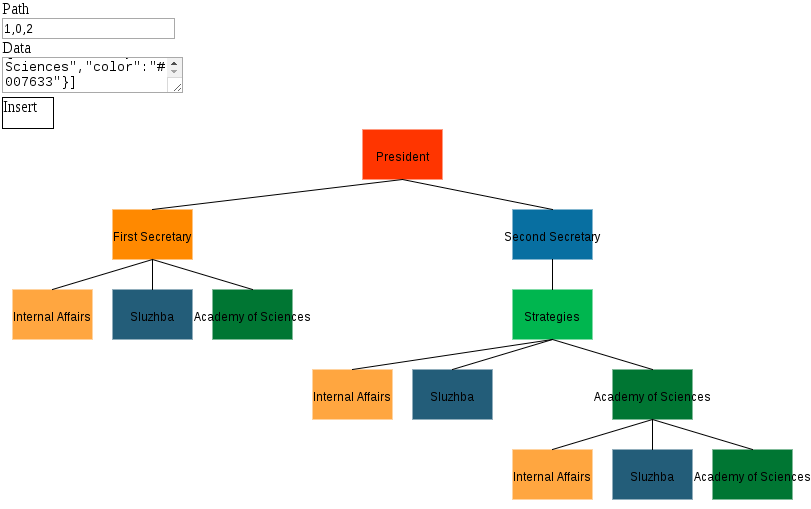
\includegraphics[width=10cm]{fig6_org_chart_vis}
\caption{A simple responsive organisation chart with our visualisation system}
\label{fig:org_chart_vis}
\end{figure}
In this demonstration, there are also interactive elements controlling the visualisation. This time the controls are for manipulation of data objects directly. The new data is an input as JSON, which is then parsed and inserted into the container for raw data. The underlying shadows receive change notification and re-calculate graphical attributes for all compartments. The whole process does not need programmatic intervention or additional programming on change propagation is required.

%\section{Organisation Evolution Chart}

% \chapter{Performance Benchmark}
% \section{Scatter Graph}
% \section{Visualisation of Big Structures}
% \section{Defficiencies}

\chapter{Conclusion}
This work has successfully solved the problem of reusability and lack of efficient mechanism for data mapping. The solution includes a data binding and processing language that systematically calculate data dependencies. The reusability issues is addressed with a new graph description language that provides basic graphing primitives that is independent of native graphics implementations and also data binding directives. This language provides easy and transparent comprehension of the chart structure and input data specifications. With shadowing, modules at each visualisation pipeline can have well-defined interfaces and thus can be separated for more flexibility and less dependencies and entanglement with other pipeline processes. These measures help end users and developers to reuse and modify existing designs and processes to fit into their various needs.

A new data binding protocol, especially shadowing, solves the problem of mapping data or intermediate data onto graphical attributes and gadgets at appropriate times. By deploying observations between data models of pipeline processes, data digestion and propagation can be handled in an automatic way. It removes a great amount of burden on users and developers who used to constantly check for the correctness and states of data. As a bonus, interactive chart designing becomes more efficient: when users tweak configurations of the chart application, the immediate feedback on the graphics front-end enables fast editing and innovations on visualisation techniques.

\section{Future Work}
There are two major tasks to be done for this work in the future. Although being a web software, since the implementation is based on JavaScript, this work can be migrated to native software like Node.js, which also support most of the JavaScript features used in this work. By extending to native application, more graphical front-ends are made available and can be more useful in context of scientific research. This is to make this work open to more potential users.

Currently this software works with native graphics directly (HTML5 Canvas) and it also provides a shim for Chart.js, so that chart designs can be wrapped into Chart.js's chart classes so that it is easier to use in a bigger application. This leads us to interest in extending the graph description language to be compatible with other graphing libraries or native graphics as well, such as SVG and its related graphing tools. This will make more chart designs available to this software.

\begin{thebibliography}{9}
\bibitem{chen01}
Chen, C., \& Paul, R. J. (2001). Visualizing a knowledge domain's intellectual structure. \emph{Computer,} (3), 65-71.

\bibitem{bostock11}
Bostock, M., Ogievetsky, V., \& Heer, J. (2011). D³ data-driven documents. \emph{Visualization and Computer Graphics, IEEE Transactions on, 17}(12), 2301-2309.

\end{thebibliography}
\chapter{Appendix}
\section{Data Binding Language}
{\em The full documentation will be compiled. }
The data binding language is to be interpreted in a given scope defined by a data model. For instance,

Operation \textbf{Access}: `key'. This access a value directly stored in the scope as a key-value pair where the key is `key'. Scopes can have a linear hierarchy, where key-value pairs can be inherited from the superior scopes. This operation will look up the entry `key' from the current scope and the superior scopes iteratively until one match is found.

Operation \textbf{Assignment}: `key1 = key2 = ... = value;'. This will assign `value' to each of the entries `key1', `key2', ... of the current context.

These operations will access and assign to data models' entries.

Arithmetic operations such as addition ({\textbf+}), subtraction (\textbf-), mulitplication (\textbf*), division (\textbf/) and modulo (\textbf\%) are also supported. Constants such as numbers, strings, undefined values (\textbf {undefined}) and null pointers (\textbf {null}) are supported as well.

Data models can be generated as well. Object and array literals can be declared in JavaScript style. For instance,
\begin{lstlisting}[language=javascript]
{
	[key]: 10,
	key2: 20, 
	'key3': 30
}
\end{lstlisting}
defines a key-value pair model whose entries are `key2' to 20, `key3' to 30 and an entry whose key equals the the `key' in the current scope, and value 10.

Advanced data models for collections can declared as well. Infinite collection of elements can be expressed as streams.

Operation \textbf{Stream}: [\textit{start} \textit[, \textit{next} \textit] \textbf{\textbar}
\textit[.. \textit{step}\textit] .. \textit[\textit{end} \textit]], creating a iterable object that can generate a series of numbers starting from `start', and interpolates the following elements either with `next' or progresses with `step' or by default progresses by one. It can stop when next value is greater than `end' or continue the series indefinitely.

We can use this construct to represent a series of natural numbers with the expression `[1 ..]', which can be useful, with additional utility to filter and select, for generating indices for collections.
\section{Graph Description Language}
\subsection{Organisation Box Chart}
\label{sec:appendix:org_box}
\begin{lstlisting}[language=xml]
<template data-bind="org_box">
<!--
	input is of type node with properties
		x: x coordinate
		y: y coordinate
-->
	<relative-layout
		data-bind-x="
			/* interpolation animation of expression `width / 2 - 25' */

			*.interpolate(${width / 2 - 25})
			.with(*.math.cubic_bezier(.4, 1.4, 0, 1))
			.duration(1500)
			.transition" y="0">
		<shape
			type="rect"
			data-bind-style="{
				x: 0,
				y: 0,
				width: 50,
				height: 50,
				fillColor: node.color or 'transparent'
			}"></shape>
		<text
			data-bind-x="-$element.textWidth / 2"
			data-bind-y="$element.textSize">
			{{ node.name }}
		</text>
	</relative-layout>
	<template data-iterate="child, index in children">
		<template data-condition="child">
			<template data-model="{
				child_x: index ? offsets[index-1] : 0,
				child_y: 60
				}">
				<!-- recursive injection of template 'org_box' -->
				<!-- which is the template this comment resides in -->
				<relative-layout
					data-bind-x="
						*.interpolate(${child_x})
						.with(*.math.cubic_bezier(.4, 1.4, 0, 1))
						.duration(1500)
						.transition"
					data-bind-y="child_y">
					<template
						data-inject="org_box"
						data-argument="child"></template>
				</relative-layout>
				<!-- relation -->
				<shape
					type="line"
					data-bind-style="
					*.interpolate(${width}, ${child_x}, ${child.width})
					.with(*.math.cubic_bezier(.4, 1.4, 0, 1))
					.duration(1500)
					.functor(
						(\t, width, child_x, child_width => {
							startX: width / 2,
							startY: 50,
							endX: child_x + child_width / 2,
							endY: child_y
						}))
					.transition"></shape>
			</template>
		</template>
	</template>
</template>
\end{lstlisting}
% \section{Data Binding Language}
% \subsection{Expressive Power}
\end{document}